\documentclass[10pt,twocolumn]{article}

\usepackage[margin=0.62in,columnsep=0.22in]{geometry}
\usepackage{times}
\usepackage{microtype}
\usepackage{booktabs}
\usepackage{amsmath}
\usepackage{amssymb}
\usepackage{graphicx}
\usepackage{xcolor}
\usepackage{tikz}
\usepackage{pgfplots}
\usepackage[numbers,sort&compress]{natbib}
\usepackage[colorlinks=true,linkcolor=blue,citecolor=blue,urlcolor=blue]{hyperref}

\pgfplotsset{compat=1.17}
\setlength{\parskip}{2pt}
\setlength{\parindent}{0.8em}
\setlength{\textfloatsep}{6pt}
\setlength{\floatsep}{6pt}
\setlength{\intextsep}{6pt}

\newcommand{\ism}{\textsc{ISM}}
\newcommand{\ar}{\textsc{AR}}
\newcommand{\cratio}{\textsc{CR}}
\newcommand{\es}{\textsc{ES}}

\title{\vspace{-1.2em}Inspectable Symbolic Compression for Long-Context Reasoning:\\A Mixed-Results Study}
\author{Anonymous Authors}
\date{}

\begin{document}
\maketitle
\vspace{-1.7em}

\begin{abstract}
We study Inspectable Symbolic Compression (\ism), a prompt-only method that
rewrites long documents as symbols, dictionary definitions, and relations.  The
result is mixed.  \ism{} structure is functionally used: semantic dictionary
damage and symbolic-structure removal both reduce accuracy.  Yet a
natural-language model summary is significantly more accurate and more
token-efficient under the same budgets, and it dominates reuse cost-accuracy.
We therefore do not claim prompt-only \ism{} is a better compressor.  The study
identifies a boundary: symbolic text written by an LLM and read by an LLM
remains in the same class as summarization.  Future work should treat \ism{} as
executable semantic IR parsed and checked outside the LLM loop.
\end{abstract}

\section{Introduction}

Prompt-compression work usually optimizes token count and retained downstream
accuracy.  We ask a narrower diagnostic question: can a compressed
representation expose meaning units that can be inspected and intervened on?
\ism{} forces the compressor to emit symbols, a short dictionary, and relations
such as precedence or exception.

The original hypothesis was that this symbolic text would be both compact and
manipulable.  The experiments preserve only the second part.  \ism{} is read
and used by the model, but it does not beat ordinary summaries as a prompt-only
compressor.

\begin{figure}[t]
\centering
\scriptsize
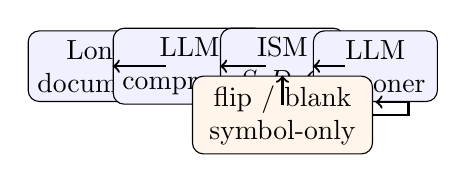
\begin{tikzpicture}[
  box/.style={draw, rounded corners, align=center, minimum width=0.62in, minimum height=0.31in, fill=blue!6},
  arr/.style={->, thick}
]
\node[box] (doc) at (0,0) {Long\\document};
\node[box] (comp) at (1.18,0) {LLM\\compressor};
\node[box] (ismn) at (2.36,0) {ISM\\$S,D,G$};
\node[box] (reason) at (3.54,0) {LLM\\reasoner};
\draw[arr] (doc) -- (comp);
\draw[arr] (comp) -- (ismn);
\draw[arr] (ismn) -- (reason);
\node[box, fill=orange!8, minimum width=0.90in] (int) at (2.36,-0.62) {flip / blank\\symbol-only};
\draw[arr] (ismn) -- (int);
\draw[arr] (int.east) -- ++(0.45,0) |- (reason.south);
\end{tikzpicture}
\caption{Prompt-only \ism{}: an LLM writes structured text and an LLM reads it
again.  This makes \ism{} directly comparable with natural-language summaries.}
\label{fig:pipeline}
\end{figure}

\section{Related Work}

\textbf{Token-level prompt compression.}
LLMLingua, LongLLMLingua, LLMLingua-2, and Selective Context compress prompts by
selecting, reweighting, or removing tokens
\citep{jiang2023llmlingua,jiang2023longllmlingua,pan2024llmlingua2,li2023selective}.
These methods are strong baselines for budgeted prompting, but the compressed
object is still an optimized prompt span rather than an explicit intermediate
representation.

\textbf{Learned memory compression.}
Gist Tokens, AutoCompressors, and ICAE replace long context with trained latent
or soft-token memory \citep{mu2023gist,chevalier2023autocompressors,ge2024icae}.
They can be compact and reusable, but their internal state is not directly
inspectable or locally editable by a human or a symbolic checker.

\textbf{Intervenable bottlenecks.}
Concept Bottleneck Models and Concept Embedding Models show why an intermediate
representation can be useful even when it is not the shortest representation:
named concepts can be inspected or intervened on
\citep{koh2020concept,espinosa2022concept}.  \ism{} imports that motivation into
prompt compression, but keeps the representation textual and prompt-only.  This
paper tests whether that textual bottleneck is enough.

\section{Method}

Each example contains a document $x_i$, questions $q_{ij}$, and labels
$y_{ij}$.  A producer $m$ writes a compressed context $z_i^m$ under budget $B$,
and the same frozen reasoner answers from that context:
\[
z_i^m(B)=P_m(x_i;B), \qquad |z_i^m(B)|_T \le B,
\]
\[
\hat y_{ij}^m = R\!\left(z_i^m(B), q_{ij}\right).
\]

\ism{} is the producer whose output is
\[
z_i^{\ism}=(S_i,D_i,G_i),
\]
where $S_i=\{Z_1,\ldots,Z_k\}$ are labels, $D_i$ maps each label to a condition
and conclusion, and $G_i$ records relations such as precedence, exception, or
conjunction.  Natural-language summary, keyword extraction, and oracle gold
summary are evaluated under the same answer protocol.

Accuracy is measured over paired questions:
\[
\mathrm{Acc}_m=\frac{1}{N}\sum_{i,j}\mathbf{1}\!\left[\hat y_{ij}^m=y_{ij}\right].
\]
We also report accuracy retention, compression ratio, and efficiency score:
\[
\ar_m=\frac{\mathrm{Acc}_m}{\mathrm{Acc}_{\mathrm{full}}}, \qquad
\cratio_m=\frac{|z_i^m|_T}{|x_i|_T}, \qquad
\es_m=\frac{\ar_m}{\cratio_m}.
\]

The ablations separate three constructs.  Derangement permutes labels while
preserving the definition multiset, conclusion flip changes the semantic
content of dictionary rules, blanking removes dictionary content, and
symbol-only/random-symbol controls test whether relations carry information
beyond arbitrary markers.

\section{Results}

\paragraph{RQ1: \ism{} structure is used.}
After correcting a low-purity compressor and replacing weak label derangement
with semantic conclusion flips, dictionary content and symbolic structure both
show functional effects.

\begin{table}[t]
\centering
\scriptsize
\begin{tabular}{lccc}
\toprule
Condition & Acc & \ar & \cratio \\
\midrule
Full Context & 0.750 & 1.000 & 1.000 \\
Full Symbol+Dict & 0.446 & 0.594 & 0.745 \\
Flipped Dict & 0.367 & 0.489 & 0.745 \\
Symbol Only & 0.413 & 0.550 & 0.079 \\
Random Symbol & 0.304 & 0.406 & 0.738 \\
\bottomrule
\end{tabular}
\caption{Dictionary ablation, dev scale-up.  $N=120$ documents, 240 questions.
Full results are in \texttt{docs/evidence/ablation-qwen7b-N120/}.}
\label{tab:rq1}
\end{table}

At $N=240$ paired questions, semantic dictionary flip is positive and
significant ($\Delta_{\mathrm{map}}^{\mathrm{flip}}=+0.079$, 95\% CI
$[0.013,0.146]$, $p=0.032$), and Symbol Only beats Random Symbol
($\Delta_{\mathrm{symbol}}=+0.108$, 95\% CI $[0.050,0.167]$, $p=5e$-$4$).
Derangement is not significant, indicating that surface label binding is not
the main mechanism.

\paragraph{RQ3: summaries beat \ism{} under fixed budgets.}
The primary analysis is paired on the same 80 questions, so it is not explained
by full-context filler degradation.

\begin{table}[t]
\centering
\scriptsize
\begin{tabular}{rccc}
\toprule
Budget & Summary-\ism{} & 95\% CI & McNemar $p$ \\
\midrule
128 & +0.2500 & [0.100,0.400] & 0.0029 \\
256 & +0.3125 & [0.175,0.450] & $1.1e$-$4$ \\
512 & +0.3750 & [0.250,0.500] & $2.3e$-$7$ \\
\bottomrule
\end{tabular}
\caption{Primary paired contrast: Model Summary minus \ism{} accuracy.  Summary
wins at every budget.}
\label{tab:paired}
\end{table}

\begin{figure}[t]
\centering
\scriptsize
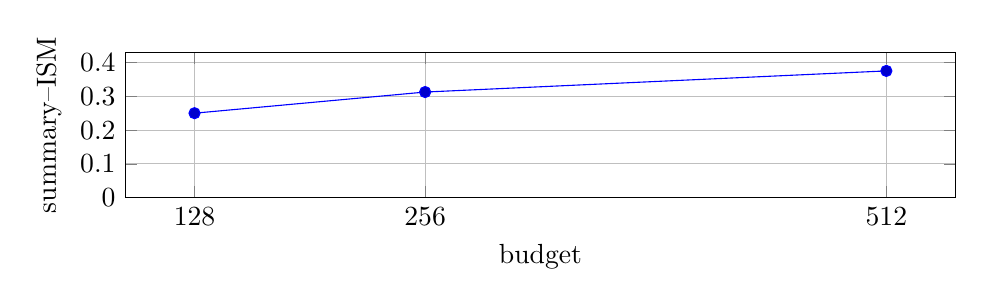
\begin{tikzpicture}
\begin{axis}[
  width=\columnwidth,
  height=1.35in,
  ymin=0,
  ymax=0.43,
  xlabel={budget},
  ylabel={summary--ISM},
  xtick={128,256,512},
  grid=major,
]
\addplot+[mark=*] coordinates {(128,0.25) (256,0.3125) (512,0.375)};
\end{axis}
\end{tikzpicture}
\caption{The paired summary advantage grows with budget in the dev pilot.}
\label{fig:summarywins}
\end{figure}

Fixed-budget \ar{}/\es{} cells show the same pattern. At budgets 128/256/512,
Model Summary reaches 1.036/51.3, 1.125/17.3, and 1.196/13.3, while \ism{}
reaches 0.679/9.4, 0.679/9.3, and 0.661/8.9.

\paragraph{RQ4: reuse is not \ism{}-specific.}
Cached representations become cheaper than full context from $n=2$ questions
onward, but Model Summary is cheaper and more accurate than \ism{}.

\begin{table}[t]
\centering
\scriptsize
\begin{tabular}{lrrrr}
\toprule
Method & $n=1$ & $n=8$ & $n=64$ & Acc \\
\midrule
Full Context & 1354 & 10828 & 86624 & 0.700 \\
Model Summary & 1526 & 2168 & 7305 & 0.787 \\
\ism{} & 1548 & 2265 & 8005 & 0.475 \\
Keyword & 1820 & 3492 & 16868 & 0.512 \\
\bottomrule
\end{tabular}
\caption{Reuse cost at budget 256.  Reuse helps all cached text, but summary
dominates \ism{} in both cost and accuracy.}
\label{tab:reuse}
\end{table}

\section{Discussion}

The positive result is that \ism{} is not inert: the model uses semantic
dictionary content and symbolic relations.  The negative result is stronger for
the original compression claim: in the prompt-only setting, \ism{} and Model
Summary are both LLM-written texts read by an LLM, and the ordinary summary is
the better text cache.

Thus the study should not be read as a successful new compressor.  It is a
boundary result.  To become categorically different from summaries, \ism{} must
be parsed, checked, transformed, and executed by programs outside the LLM.  The
future claim is not ``summaries cannot be edited'' but ``semantic IRs permit
automatic, local, schema-validated edits and symbolic execution.''

\section{Limitations}

The reported experiments are dev-scale and synthetic.  QASPER
\citep{dasigi2021qasper} and LLMLingua-2 are specified but not fully evaluated
here.  Several large GPU artifacts are stored by sha256 and reproducibility
commands.  RQ2 dictionary swap remains future work.  Most importantly, this
paper evaluates prompt-only \ism{}, not a parser/checker/executor system.

\section{Conclusion}

\ism{} representations are functionally used, but prompt-only \ism{} is not a
better compressor than natural-language summaries.  This mixed result closes
one path and clarifies the next: executable semantic IR for long-context
reasoning.

The boundary claim is precise: structured prompt text can expose units that an
LLM uses, but it does not by itself create a new computational object.  The next
version must make the representation parseable, checkable, and executable by
ordinary software.

\section{Pre-registered Status}

\begin{table}[t]
\centering
\scriptsize
\begin{tabular}{lll}
\toprule
Criterion & Status & Evidence \\
\midrule
\#1 \ism{} $>$ Summary & Failed & RQ3/RQ4 summary dominates \\
\#2 structure used & Met & flip $p=0.032$; symbol $p=5e$-$4$ \\
\#3 unseen swap & Open & LoRA swap not run \\
\bottomrule
\end{tabular}
\caption{Dev-scale status of the original criteria.  Since criterion \#1 fails,
we do not claim an efficiency advantage for \ism{}.}
\label{tab:status}
\end{table}

Criterion \#2 supports functional use of the internal structure, but that is
distinct from being a better compressor.  The original efficiency hypothesis is
not supported.

\section{Semantic-IR Path}

\begin{table}[t]
\centering
\scriptsize
\begin{tabular}{lll}
\toprule
Property & Summary & Semantic IR \\
\midrule
Format & free text & schema / AST \\
Validation & manual & checker \\
Edit & rewrite & rule-id local edit \\
Execution & LLM & symbolic executor \\
\bottomrule
\end{tabular}
\caption{The path that would make symbolic compression categorically different
from summaries.}
\label{tab:ir}
\end{table}

The next research question is compile-and-execute: can an LLM compile a long
document into an IR that a non-LLM program can parse and run?  That would make
the representation categorically different from a short natural-language
summary.

\section{Evidence Ledger}

\begin{table}[t]
\centering
\scriptsize
\begin{tabular}{lll}
\toprule
Finding & Evidence & Status \\
\midrule
\ism{} is used & ablation-qwen7b-N120 & positive \\
Summary wins & fixed-budget-N40 & negative \\
Reuse not unique & reuse-N40 & negative \\
Root cause & llm-ism-diagnostic & resolved \\
\bottomrule
\end{tabular}
\caption{The mixed result is internally consistent: the representation carries
signal, but the prompt-only implementation loses the efficiency contest to a
plain summary.}
\label{tab:ledger}
\end{table}

\section{Next Tests}

\textbf{Compile-and-execute.} Convert \ism{} text into a schema-checked AST and
answer with a deterministic executor.  \textbf{Targeted edits.} Repair or delete
a rule by id and verify the prediction changes locally.  \textbf{Swap.} Finish
the LoRA dictionary-swap experiment for unseen labels.

\section{Reproducibility}

Evidence is stored under \texttt{docs/evidence/}: \texttt{ablation-qwen7b-N120}
for RQ1, \texttt{fixed-budget-N40} for RQ3, \texttt{reuse-N40} for RQ4, and
\texttt{llm-ism-diagnostic.md} for the corruption/purity diagnosis.  Large GPU
outputs are retained by sha256 and reproducibility commands.

\section*{References}
\scriptsize
\begin{thebibliography}{10}
\bibitem{koh2020concept} Koh et al. Concept Bottleneck Models. ICML 2020.
\bibitem{espinosa2022concept} Espinosa Zarlenga et al. Concept Embedding Models. NeurIPS 2022.
\bibitem{dasigi2021qasper} Dasigi et al. A Dataset of Information-Seeking Questions and Answers Anchored in Research Papers. NAACL 2021.
\bibitem{jiang2023llmlingua} Jiang et al. LLMLingua. EMNLP 2023.
\bibitem{jiang2023longllmlingua} Jiang et al. LongLLMLingua. ACL 2024.
\bibitem{pan2024llmlingua2} Pan et al. LLMLingua-2. Findings ACL 2024.
\bibitem{li2023selective} Li et al. Compressing Context to Enhance Inference Efficiency of LLMs. EMNLP 2023.
\bibitem{mu2023gist} Mu et al. Learning to Compress Prompts with Gist Tokens. NeurIPS 2023.
\bibitem{chevalier2023autocompressors} Chevalier et al. Adapting Language Models to Compress Contexts. EMNLP 2023.
\bibitem{ge2024icae} Ge et al. In-context Autoencoder for Context Compression in a Large Language Model. ICLR 2024.
\end{thebibliography}

\end{document}
